\section{GUI}\label{gui}

Die GUI (\textit{graphical user interface}) wurde mit Android und den GooglePlay Services (einschlie�lich Google Maps) umgesetzt. 
Die mitgelieferten
M�g\-lich\-kei\-ten des Android SDK sind in dieser Hinsicht f�r die GUI-Umsetzung dieses Projektes vollkommen zufriedenstellend. Die komplette
GUI setzt sich aus zwei Activities zusammen, die im Folgenden n�her betrachtet werden.

\subsection*{Login-Screen}
Diese Activity wird zuerst aufgerufen und zeigt einen Bildschirm auf dem sich der Spieler einen Benutzernamen aussucht und danach mit dem
"`Start"' Button zu n�chsten Activity wechselt, welche das eigentliche Spiel zeigt (siehe Abbildung \ref{fig:chat}).

\begin{figure}
    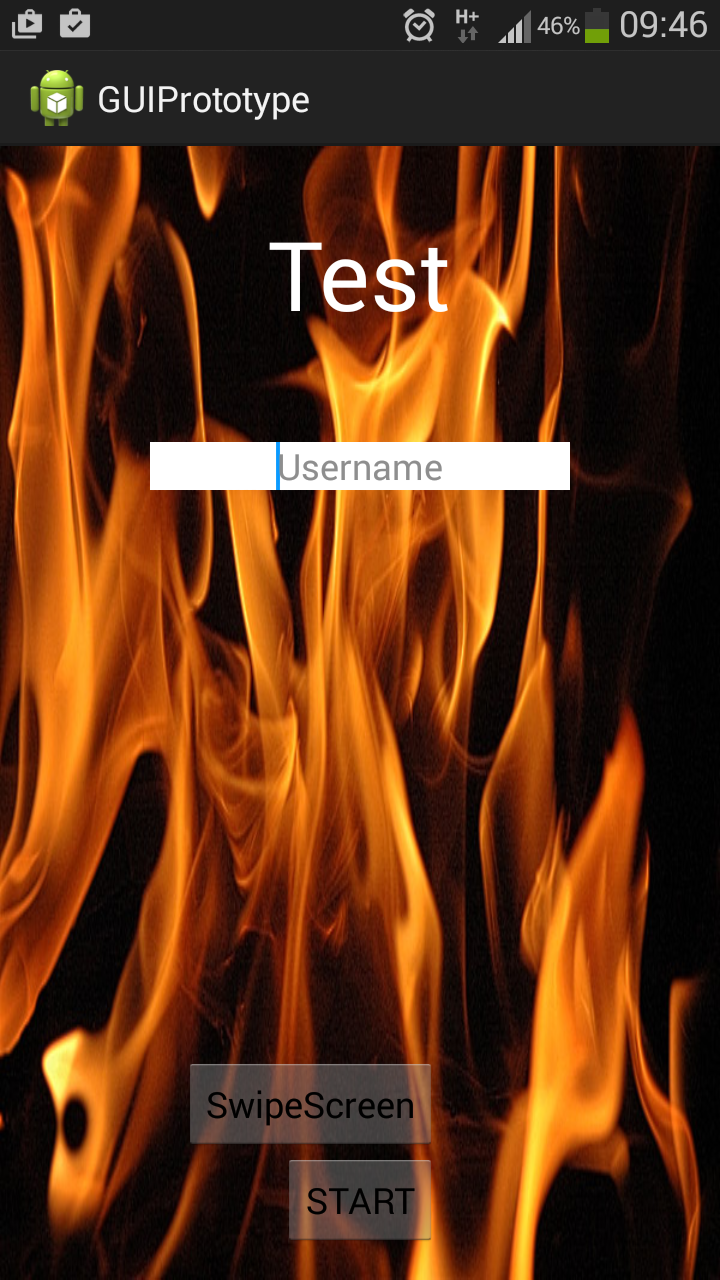
\includegraphics[width=0.5\textwidth]{4-Technische_Loesungen/4-5-GUI/Data/login_screen.png}
    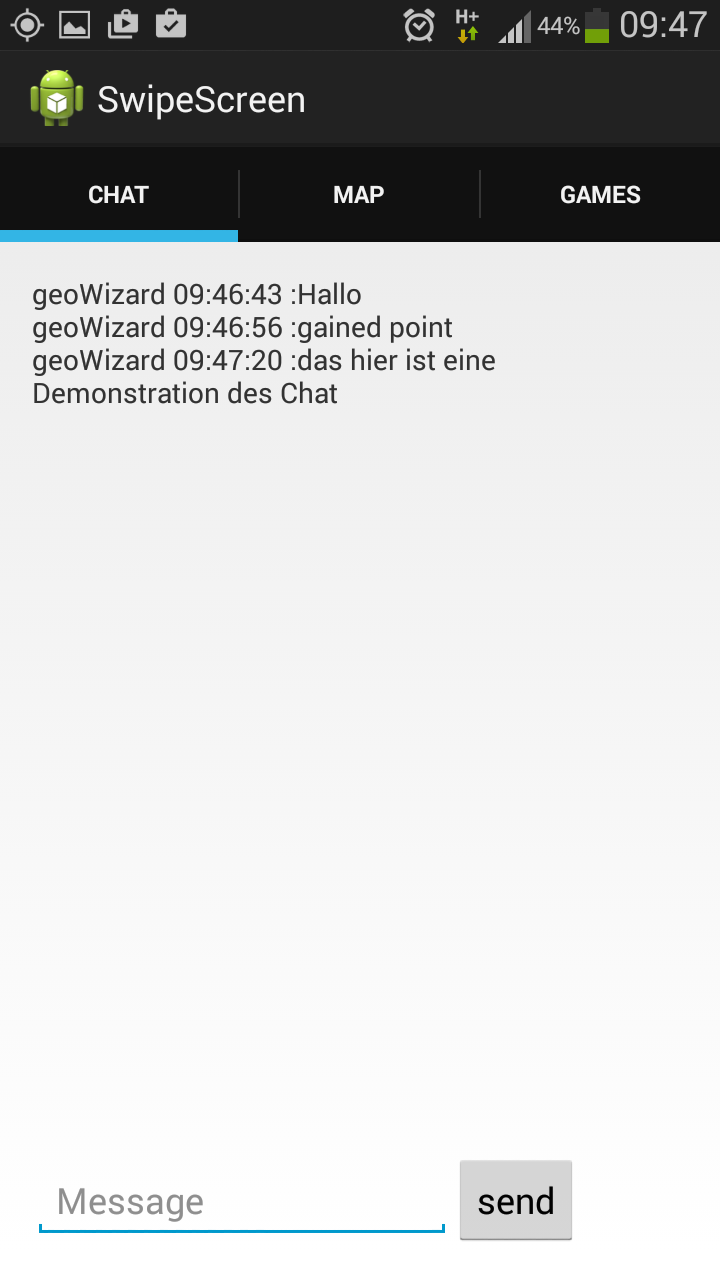
\includegraphics[width=0.5\textwidth]{4-Technische_Loesungen/4-5-GUI/Data/chat_screen.png}
     \caption{Login-Screen (rechts) und Chat-Screen (rechts)}
     \label{fig:chat}
\end{figure}


\subsection*{Swipe-Screen}
Schon in der sehr fr�hen Entwicklungsphase war festzustellen, das die verschiedenen Elemente der GUI, wie im folgenden weiter erl�utert, zu zahlreich sind, um sie auf einen Bildschirm umzusetzen. Die eigentliche Kartendarstellung w�re sonst zu klein gewesen. Also wurde entschieden die verschiedenen Elemente auf weitere Bildschirme zu verteilen. In den ersten Entw�rfen geschah dies �ber einzelne Activities, also mehrere Voll\-bild-Fens\-ter. Um gewisse Android Kom\-fort-Funk\-tio\-nen und Gesten dem Nutzer zu verf�gung zu stellen wurden die zun�chst eigenst�ndigen Activites zu Fragments umgebaut, die dann in einem so genannten Swipe-Screen zusammengefasst werden. In diesem werden die Fragments als Tabs organisiert und der User kann entweder durch "`wischen"' (\textit{swipe}) oder durch klicken auf die Tabs durch die GUI Navigieren. 

Ein weiterer Vorteil ist ebenfalls, dass benachbarte Tabs jeweils vorgeladen (Laden der Widgets) und noch im Speicher behalten werden. Zum einen wird so sichergestellt, dass der Tab-Wechsel durch Wischen "`geschmeidig"' abl�uft. Dadurch ergeben sich auch  geringere Ladezeiten zwischen den einzelnen Bildschirmen. Zudem ist die  "`Wiederverwendbarkeit"' von Fragments als UI (\textit{user interface}) ebenfalls n�tzlich, wenn weitere �hnliche Spiele umgesetzt werden sollen. Der Swipe-Screen umfasst drei Tabs: Der Map-Screen zeigt den aktuellen Spielzustand, �ber den Chat-Screen k�nnen sich Spieler einer Spielinstanz austauschen und der Game-Screen erlaubt es, eine neue Spielinstanz zu erstellen oder einer bestehenden Spielinstanz beizutreten. 


\subsection*{Chat-Screen}
In desem Fragment wird die M�glichkeit des Chattens zwischen mehreren Spielern umgesetzt (siehe Abbildung \ref{fig:chat}). Die grafische Umsetzung des Chats wurde der von IRC (Instant Relay Chat) Clients nachempfunden und ist entsprechend simpel gel�st. Es wird der jeweilige Benutzername, Uhrzeit und die eigentliche Nachricht angezeigt. Die Eingabe der Chat-Nachricht erfolgt in einem Text-Eingabe-Feld. Die Anzeige der Chat-Nachrichten erfolgt in einem einfachen Textanzeige-Feld (TextView\footnote{{\url{http://developer.android.com/reference/android/widget/TextView.html}}}) was wiederum in einem scrollbaren Feld (SrcollView\footnote{\url{http://developer.android.com/reference/android/widget/ScrollView.html}}) liegt. Hierdurch ist es m�glich den Nachrichtenverlauf zu durchsuchen. Wird eine Chat-Message (genaueres in Kapitel 4.4) empfangen, wird diese an das Textfeld angeh�ngt. Hierbei ist zu beachten, dass die selbst verschickten Nachrichten erst an den Server gesendet werden und dann jeweils an die entsprechenden Nutzer. Dabei muss eine gringe �ber\-tra\-gungs\-ver\-z�\-ge\-rungen in Kauf genommen werden, jedoch ist die korrekte Reihenfolge der Nachrichten ge\-w�hr\-leis\-tet.


\begin{figure}
    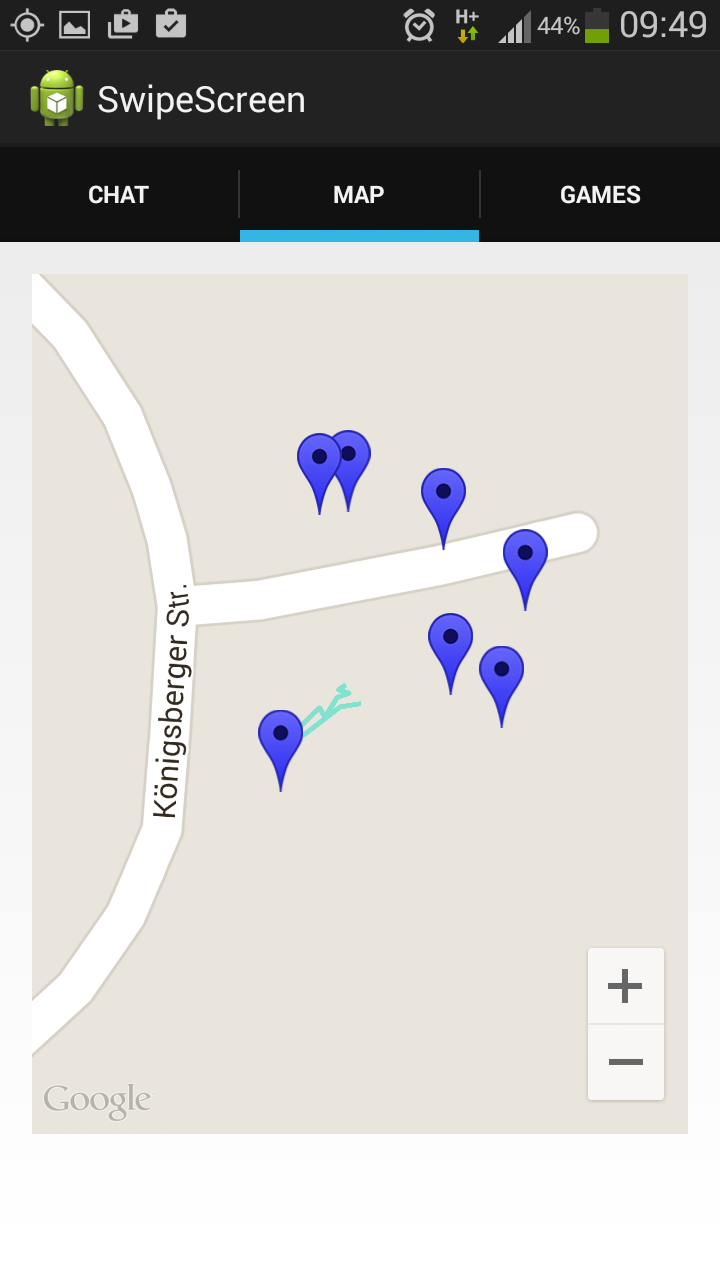
\includegraphics[width=0.5\textwidth]{4-Technische_Loesungen/4-5-GUI/Data/map_screen.png}
    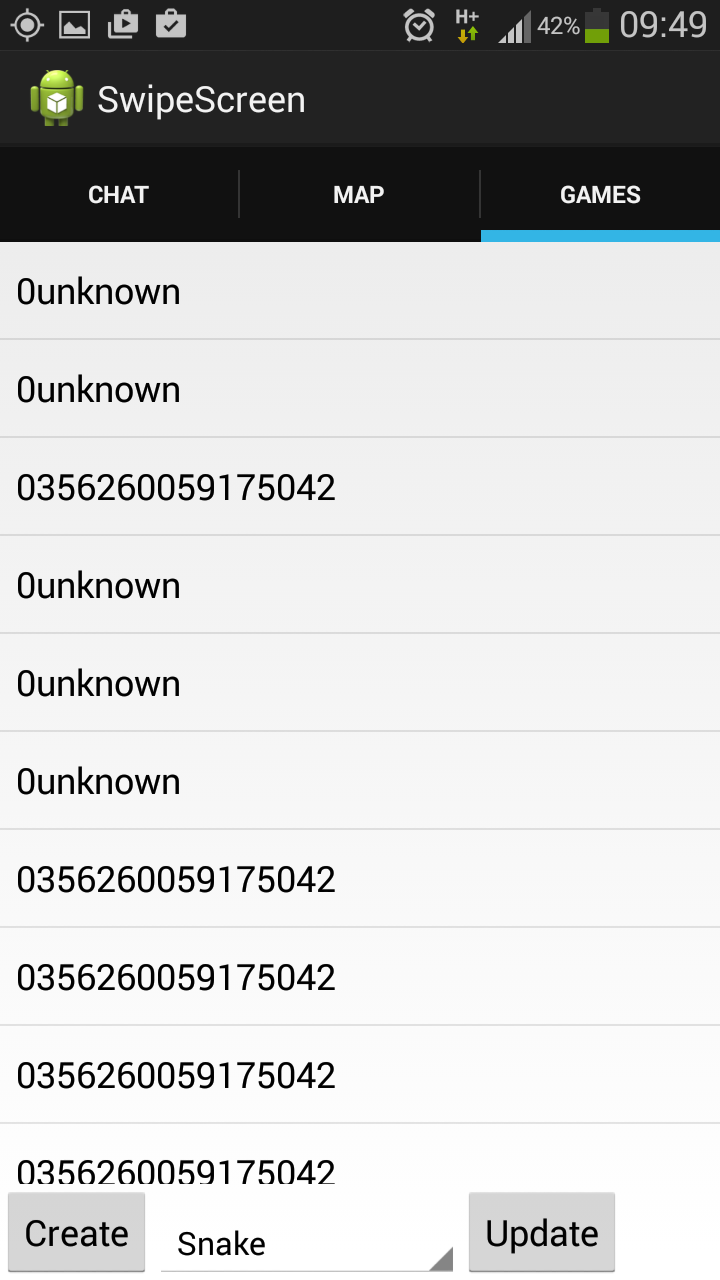
\includegraphics[width=0.5\textwidth]{4-Technische_Loesungen/4-5-GUI/Data/game_screen.png}
         \caption{Map-Screen (links) und Game-Screen (rechts)}
         \label{fig:game}
\end{figure}

\subsection*{Map-Screen}
In diesem Fragment wird die Karte der n�heren Umgebung des Spielers dargestellt (siehe Abbildung \ref{fig:game}). Auf der Karte werden alle in der aktuellen Spielinstanz vorhandenen und f�r den Spieler sichtbaren virtuellen Objekte und Mitspieler angezeigt. Je nachdem welches Spiel gespielt wird sind zus�tzliche In\-ter\-ak\-tions\-m�g\-lich\-kei\-ten und Anzeigefelder vorhanden, wie beispielsweise die Anzeige des Punktestands der Teams.


\subsection*{Game-Screen}
In diesem Fragment werden momentan aktive Spielinstanzen angezeigt (siehe Abbildung \ref{fig:game}). Auch ist es m�glich neue Spiele zu erstellen. Die Anzeige der Liste der Spiele erfolgt in einer scrollbaren Liste (ListView). Diese wird regelm��ig aktualisiert. Die Listen-Elemente sind interaktiv: Ein klick auf das entsprechende Spiel startet den Beitritt. Um ein Spiel eines gewissen Typs zu Starten w�hlt man in einen Drop\-down-Men� (bei Android Spinner) den entsprechenden Modus aus in klickt auf \glqq Create\grqq. Man selbst betritt dieses Spiel und der Eintrag in der Spiele-Liste wird vorgenommen. 

\subsection*{Haptisches Feedback}
Die graphische Benutzeroberfl�che kann durch Haptisches Feedback erg�nzt werden. Haptisch bedeutet \glqq f�hlbar\grqq oder \glqq ber�hrbar\glqq. Bei Smartphones betrachten wir in diesem Zusammenhang den Vibrationsalarm. Dieser wird nativ dazu genutzt um dem Nutzer mitzuteilen, dass ein Anruf oder eine Nachricht eingegangen ist oder um Eingaben zu best�tigen.
Erzeugt werden die Vibrationen durch einen kleinen Motor, der durch eine Unwucht daf�r sorgt, dass das Geh�use vibriert. Bei einigen Ger�ten wird sogar der Lautsprecher dazu genutzt, indem er niedrigfrequente T�ne erzeugt, die das Geh�use in Schwingung versetzen.


